\documentclass[../Main/Knit.tex]{subfiles}

\newpage
\section{Iso-Seq: Bioinformatics Pipeline} 
While the official PacBio bioinformatics tool (Iso-Seq) has been revised multiple times during the scope of this PhD, there are two main steps with the aim of generating high-quality (HQ) isoforms de novo (Figure X), namely: 
\begin{itemize}
	\item Classify to identify full-length non-chimeric (FLNC), and non-FLNC reads 
	\item Cluster reads derived from the same isoform to generate consensus sequence	
\end{itemize}
Bioinformatic analysis of Iso-Seq raw data can be performed using PacBio SMRT Link Suite (ref), a web-based end-to-end user interface. However, for optimisation of parameters and parallelisation of samples, an end-to-end command line was developed and used. Since the development of Iso-Seq, a myriad of bioinformatics tools have been released, as outlined in Table X. 

\begin{figure}[h!]
	\centering
	\vspace{20pt}
	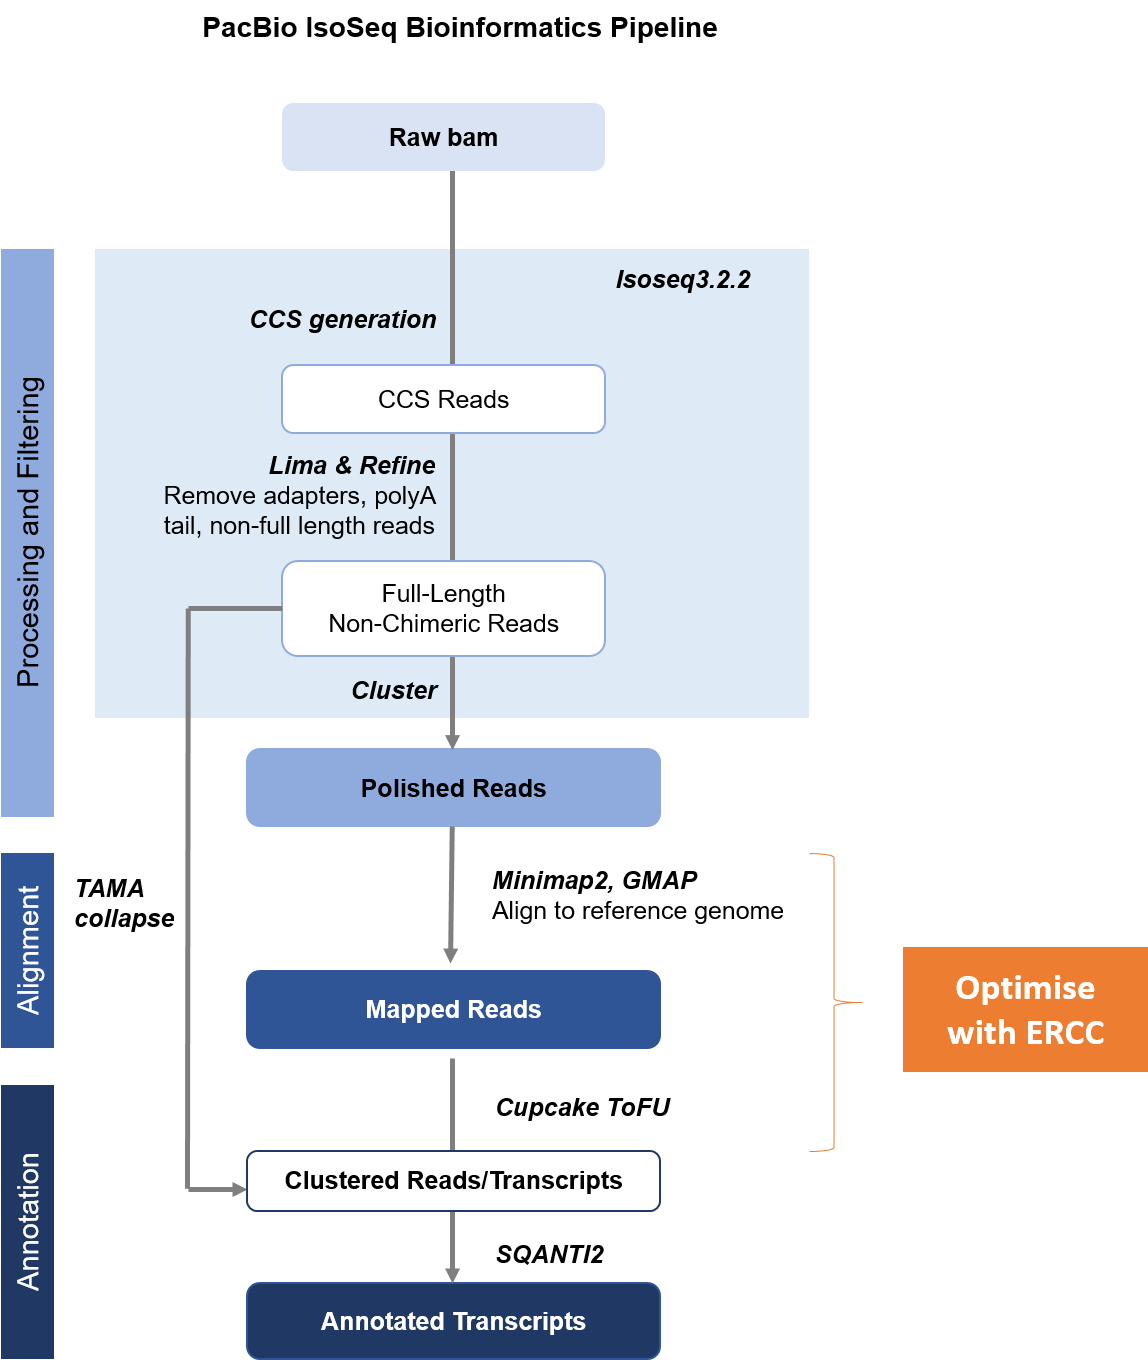
\includegraphics[width=0.8\linewidth, height=0.6\textheight]{Pictures/Isoseq_Pipeline.png}
	\captionsetup{width=0.95\textwidth}
	\caption[PacBio Isoseq Bioinformatics Pipeline]%
	{\textbf{PacBio Isoseq Bioinformatics Pipeline}: Pipeline is adapted from ToFU \nomenclature{ToFU}{Transcript isOforms: Full-length and Unassembled} \cite{Gordon2015}}
	\label{fig:isoseq_bioinformatics_Pipeline}
\end{figure}

Analysing long-read sequencing data requires a different approach to short-read, as the initial processing focuses on reducing the high error rate (due to low read coverage relative to short reads). Currently there are three methods of correcting long reads \cite{Zhao2019}: 
\begin{itemize}
	\item Hybrid error correction strategy using short-reads: LSC \cite{Au2012} which maps short reads, and LoRDEC which build De Brujin graph of short reads \cite{Salmela2014}
	\item Self-correction using long reads only: Long-read multiple aligner (LoRMA) \cite{Salmela2017}
	\item Reference-based correction by alignment of reads to reference genome by spliced-aware aligners: Minimap2. GMAP and STAR can also be used for alignment, however, they do not perform error correction during alignment and further capture non-canonical splice sites.  
\end{itemize}

Although the raw error rate of PacBio sequencing is 10-14\%, this is greatly reduced by the use of circular template and subsequent generation of circular consensus sequence. 

\subsection{ERCC}
One source of error from long-read sequencing can occur at reverse transcription, whereby a premature termination in reverse transcription enzyme can result in a full-length cDNA, that is mistaken for a true isoform. To measure the degree of this technical error, ERCC, with known start and end positions can be used as benchmark. As detailed in \cite{Karlsson2017}, most ERCC reads fell within +/- 5bp at both 5' and 3' ends, with 3' end slightly more accurate than 5' end. From \cite{Sharon2013}, drop in read length was observed for ERCC for molecules longer than 1.5kb (PacBio RSII). Interestingly, non-coding exon junctions were more variable than coding-exon junctions, suggesting that codon exon splicing has a stricter control with refined splice donor/acceptor sites (\citep{Karlsson2017}) 
Of note, however, that while ERCC has been used as a standard for RNA-Seq method validation, the longest molecule is only ~2kB, thus limiting is usage to validate longer molecules. Given that XX of RNA transcripts in human and mouse transcriptome are >2kB, there is a need for longer control sequences. 


\subsection{Classify}
\label{section:classify}

\uline{\textbf{CCS Generation}}: In the first stage, the raw subreads (stored as a BAM file, unaligned.bam) from each “productive” ZMW are processed individually and collapsed to generate a CCS (Figure \ref{fig:CCS}), according to: 
\begin{itemize}
	\item The number of full "passes" from the polymerase, and subsequently number of subreads generated; a full pass is defined by the presence of both SMRT adapters at both ends (Default: 3 passes)
	\item The minimum base accuracy across all subreads (Default: 99\%)
	\item Length of the subreads (Default: minimum 10 bases, maximum 21000 bases)
	\item Quality of Subread predicted by the CCS model (Default: Z-score of -3.5), and proportion of total subreads meeting the quality score (Default: \textgreater 30\%)
\end{itemize}

Across literature and PacBio scientific community, different parameter settings were recommended, particularly with \textit{number of full passes} and \textit{minimum base accuracy}, which had the greatest effect on the number of CCS reads generated for downstream analyses. Taking a subset of raw data from 10 randomised samples, a range of values across these two parameters were tested. CCS are then classified to full-length (FL, determined by the presence of 3'/5' primers and poly-A tail) and non-full-length (NFL) reads. 

\uline{\textbf{Lima}}: With successfully-generated CCS, cDNA primers and PacBio barcodes are identified and then removed using lima. CCS with unwanted orientations are removed and are oriented 5’ to 3’. A barcode score is calculated for each barcode pair (leading and trailing barcode), and is based on accuracy alignment to input cDNA primer sequences. The proportion of FL reads (number of FL reads over the number of CCS reads) varies on the insert transcript size; for Iso-Seq, a non-size selected library with a library distribution of 1-3kB typically has a 60-70\% FL. 

\uline{\textbf{Refine}}: Finally, full-length reads are refined by trimming of polyA tails, of a least a length of 20 bases, and removal of artificial concatemers to generate full-length non-chimeric (FLNC) reads. Artificial concatemers are defined as cDNA sequences with internal runs of polyA and polyT sequences, due to insufficient amount of blunt adapters during library preparation - this is typically rare (<0.5\%). Conversely, it is challenging to differentiate and remove PCR-induced artificial chimera from true biological chimera. PCR-induced artefacts are defined as cDNA sequences that appear to be fusion transcripts, but are actually a result of non-optimal PCR reaction conditions. The number of FLNC reads should be very close to the number of FL reads, and any significant loss implicates issues at the SMRT bell library preparation.
Note Tama works on FLNC reads from Classify 

\subsection{Cluster}
In the second stage, Iso-Seq uses an iterative isoform-clustering algorithm (ICE – iterative clustering for error, called Quiver for PacBio RSII data and Arrow for PacBio Sequel data) to group all FLNC reads that are thought to be derived from the same isoform if: 
\begin{itemize}
	\item They differ less than 100bp on the 5’ end 
	\item Differ less 30bp on the 3’end 
	\item Do not contain internal gaps that exceed 10bp
\end{itemize}
By collapsing transcripts with differing 5' start [due to cDNA synthesis not preserving 5' end], some transcripts with alternative transcription start sites are lost while preserving those with alternative splicing and alternative polyadenylation. The representative transcript from those clustered is the longest one. 

A minimum of two FLNC reads are further required for a cluster. Two possible issues: reads belong to incorrect clusters, and reads that belong together are in separate clusters. [Briefly it first does clique-finding based on a similarity graph, then calls consensus using the Directed Acyclic Graph Consensus method and finally reassign sequences to different clusters based on their likelihood (Gordon et al. 2015)]. In previous Iso-Seq bioinformatic versions, NLF reads were used to increase the coverage of each consensus isoform. However, with increasing throughput with Sequel I and Sequel II, this has been foregone. Cluster outputs the high-quality isoforms (HQ-isoforms), which have a consensus accuracy >=99\%. 

So in summary, each productive ZMW generates one polymerase read, which is collapsed to give a circular consensus sequence (CCS) assuming the requirements are met. CCS are then trimmed and processed for primer and poly-A sequence removal to generate full-length non-chimeric (FLNC) reads, which are clustered if they are thought to be derived from the same isoform. The number of associated full-length (FL) reads of each isoform therefore represents the number of ZMWs that sequenced the isoform of interest, and can infer abundance of mRNA isoform. However, Iso-Seq is only semi-quantitative due to preferential loading and sequencing bias of shorter fragments. It is worthy to note that all the steps up to now have een processed without a reference genome or transcriptome. 


Iso-Seq Versions 
In response to a much higher experimental throughput of Sequel compared to RSII, each subsequent   version of the official PacBio Iso-Seq tool saw a reduction in runtime, but an improvement of sensitivity to recover transcripts and specificity to reduce artefacts.

Iso-Seq 1 	
Iso-Seq 2	


In previous versions of official PacBio IsoSeq tool, non-FLNC reads are re-incorporated at this stage to polish the consensus isoforms. Short reads from RNA-Seq can also be incorporated for error correction using various tools such as LoRDEC, LSC and Proovread. 

Since the introduction of Iso-Seq protocol, 3 versions of the informatics pipeline has been developed. Iso-Seq2 has an extra pre-clustering step to bin full length non-chimeric reads based on gene families. The latest version Iso-Seq3 is used in response to the much higher throughput of Sequel compared to RSII by using faster clustering algorithms. Using a more conservative primer removal and barcode demultiplexing step (with tool named LIMA), the Iso-Seq3 pipeline generates fewer but higher quality polished transcripts. 

High confidence transcripts can be determined by 1) presence of open reading frame (ORF), CDS length, interpro domain coverage, annotation edit distance 

\subsection{Genome/Transcriptome Alignment} 
High quality isoforms are then aligned to the reference genome (as opposed to transcriptome as otherwise miss novel isoforms using BLASR) using splice-aware aligner Minimap2. Various long-read studies have used Minimap2 and GMAP (Križanovic et al. 2018 demonstrated marked success of GMAP vs other RNA-Seq Aligners). Tang et al. 2020, using subset of Oxford Nanopore reads evaluated number of splice sites mapped relative to known junctions, found Minimap2 to be more precise than GMAP. 

Using the –secondary=no parameter restricts the output to the best alignment, -x splice assumes read orientation relative to transcript strand unknown, and thus tries two rounds of alignment to infer orientation. As a splice-aware alignment, -x splice prefers GT[A/G]…[C/T]AG over GT[C/T]…[A/G]AG over other splicing signals (main donor/acceptor motifs). –u f forces minimap2 to consider forward transcript strand only for alignment, slightly improving accuracy. –c 5 to accept non-canonical GT/AG splice junctions. 

--splice-flank=yes for human/mouse data in reads with relatively high sequencing error rate (necessary for ONT), but not for high quality IsoSeq reads (99\% - 100\%). 

\subsection{Genome Mapping}
HQ-isoforms from the pooled dataset were aligned to mouse genome using Minimap2, and a total of XXX reads (XX\%) were mapped. Errors for substitution, insertion and deletion are X\%, X\% and X\% respectively. XX\% of transcripts (polished) could not be mapped to reference genome, thus representing genes that fall into gaps in the assembly (mouse genome should be quite updated though)


\subsection{Cupcake}
To avoid redundancy of transcripts, aligned and filtered HQ transcripts are further collapsed to obtain a final set of unique, full-length, high-quality isoforms using Cupcake (a set of publicly-available, supporting scripts). HQ transcripts are filtered out for lack of mapping and low coverage/identity before collapsing into unique isoforms.  

The abundance of each unique isoform can be estimated from the number of associated FL and NFL reads during IsoSeq cluster (not accounting for HQ transcripts that have been filtered out).  Finally, isoforms are filtered by 5’degradation due to the lack of a cap protection employed in the cDNA synthesis step (Clontech SMARTer cDNA kit). 


\subsection{SQANTI2} 
High-quality, clustered, filtered isoforms from Cupcake are characterised using SQANTI2, a pipeline initially developed by Conesa et al. [ref] and refined by Elizabeth Tseng (Pacific Bioscience’s specialist) [ref]. In addition to providing the descriptive statistics for each transcript (such as the chromosome, the strand, the length and the number of exons), it further allows input of public datasets and RNA-Seq data to further characterise and validate isoforms from Iso-Seq:
\begin{itemize}
	\item FANTOM5 Cap Analysis of Gene Expression (CAGE): map transcripts, transcription factors, transcriptional promoters and enhancers [ref]
	\item Intropolis: a comprehensive human RNA-Seq dataset [ref]
	\item PolyA motifs 
	\item Aligned RNASeq (Section X)
\end{itemize}


SQANTI2 pipeline involves: 
\begin{enumerate}
	\item Performs a reference-based correction of sequences [check??]
	\item Generates gene models and classifies transcripts based on splice junctions (See Section X)
	\item Predicts Open Reading Frames (ORF) for each transcript
	\item Remove isoforms potential to be artefacts
\end{enumerate}

\subsubsection{SQANTI2 classification of isoforms}
Using SQANTI classifications based o splice junctions, the transcriptome can be segregated into: 
\begin{itemize}
	\item Well-known annotated genes with known transcripts, further classified as
	\begin{itemize}
		\item Full Splice Match (FSM) if reference and query isoform have the same number of exons with matching internal junction. The 5’ and 3’ end, however, can differ 
		\item Incomplete Splice Match (ISM) if query isoform has fewer 5’ exons than the reference, but the 3’ exons and internal junctions match. The 5’ and 3’ end can also differ 
	\end{itemize}
	\item Well-known annotated genes with novel transcripts 
	\begin{itemize}
		\item Novel in Catalog (NIC) if query isoform has different number and combination of exons to reference isoform, but is using a combination of known donor/acceptor splice sites 
		\item Novel Not In Catlog (NNC) if query isoform has different number and combination of exons to reference isoform like NNC, but also has at least one unannotated/novel donor or acceptor site
	\end{itemize}
	\item Unannotated, novel genes with novel transcripts 
	\item Others
	\begin{itemize}
		\item Antisense: the query isoform does not have overlap a same-strand reference gene but is anti-sense to an annotated gene.
		\item Genic Intron: the query isoform is completely contained within an annotated intron.
		\item Genic Genomic: the query isoform overlaps with introns and exons.
		\item Intergenic: the query isoform is in the intergenic region
	\end{itemize}
\end{itemize}

Lastly it can provide further classification of transcripts:  
As protein-coding or non-protein-coding by the presence of coding sequence
that may potentially undergo non-sense medicated decay by the presence of ORF but CDS ends before the last junction
that contain one or multiple exons (mono-exonic or multi-exonic respectively)
that contain intronic sequences (intron retention) 
as fusions. The criteria XXXX

\subsection{Isoform expression from Iso-Seq} 
To control for sequencing bias in library depth, full-length (FL) read count for each isoform is normalized to transcripts per million (TPM \nomenclature{TPM}{Transcripts per Million})), which is calculated as: 

\begin{equation}
FL\;\:TPM (x_{sample},y_{sample})=\frac{Raw\;\:FL\;\:count (x_{isoform},y_{sample})}{Total\;\:FL\;\:count (y_{sample})} *10^6
\end{equation}

With a cut-off lower than 0.5 TPM, a 0.5 - 10 TPM refers to low expression, a 11- 1000 refers to medium expression, and > 1000 TPM high expression [literature ref]. 

TPM is the most effective within-sample normalisation method to relatively quantify gene expression in a sample \cite{Abrams2019}. Other methods include RPKM (reads per kilobase of transcripts per million mapped reads), FPKM (fragments per kilobase of exon model per million mapped reads), which uses gene length to control for fragmentation in RNA-Seq protocol ("effective length normalisation") - however, this is not necessary in Iso-Seq.  

Between-sample normalisation methods to relatively quantify expression of the same gene in different samples, remove technical variations due to presence of few highly expressed genes that make up a significant proportion of total reads, and due to different number of reads in each sample. 


\subsection{Validation of isoforms with RNASeq} 
Samples sequenced with paired-end reads, Illumina Hi-Seq, 125bases. Paired end reads as more accurate for identifying and sequencing junctions. RNASeq data through stringent filtering (plot of fastqc) and aligned to mouse genome (Gencode, version X) using STAR (see section X for parameters). Abundance in TPM was then calculated with Kallisto (ref) as an input into SQANTI to identify coverage of splicing junctions with RNASeq.  

Provides support of transcripts from RNA-Seq data, highest expression of RNA-Seq reads of the splice junctions 
The junction with lowest coverage from RNA-Seq, and its associated read count 	
Standard deviation of read counts across all the junctions for each transcript 

\subsection{SQANTI2 filtering}
This was developed to remove artifacts from library preparation: i.e. intrapriming of polyA that usually happens in antisense strands and also lack of junction support in NNC; increase \% of FSM transcripts, and removes NIC. 

SQANTI2 further filters isoforms, based on the following rules: 
\begin{enumerate}
	\item FSM with a reliable 3’ end by:
		\begin{itemize}
			\item >60\% of As in transcription termination site and no detected polyA motif, indicative of genomic contamination
			\item <Xbp 5' start and 3’ end to reference transcript start end
		\end{itemize}
	\item Any other transcripts that have a reliable 3' end do not have any splice junctions are annotated as Reverse Transcription Switching. 
\end{enumerate}


Reverse Transcription switch is determined on a junction level on both plus and minus strands by aligning each splice junction to reference file (splice junction defined as 3’/end of the exon to the 3’/end of the intron). The transcript is considered to be an artifact of reverse transcription if any of the junctions are labelled as RT switch. 

all junctions are either canonical or has short read coverage ( > 3 reads)

\subsection{Quantification of human transgene expression}
As reported in \cite{Castanho2020}, human-specific MAPT sequence was selected from a 2kb region present in the 3'UTR after using BLAT to identify divergent sequence in human and mouse MAPT. Counts of this human-specific MAPT sequence in the CCS and polished reads from WT and TG were then plotted as a ratio of unique reads to the total number of input reads.  

\subsection{Classification of Alternative Splicing Events}
SUPPA2 was used to classify alternative splicing events with the parameter –f ioe in isoforms retained from SQANTI2 filter. Splicing events included Alternative 5’ Splice Sites (A5), Alternative 3’ Splice Sites (A3), Alternative First Exons (AF), Alternative Last Exons (AL), Mutually Exclusive Exons (MX), Retained Intron (RI), Skipping Exon (SE). 

\subsection{Limitations}
While PacBio's Iso-Seq have major potential for transcriptome annotation, there are currently several major limitations that need to be addressed with further development of library preparation and bioinformatic data analyses \cite{Kuo2017}: 
\begin{enumerate}
	\item Lack of normalisation of RNA libraries, resulting in biased sequencing of high abundance transcripts and subsequent over-representation of such transcripts 
	\item Degradation of transcripts from 5' end, and thus lack of confidence in transcription start site and full-length structure 
\end{enumerate}


	 